\chapter{Исследовательский раздел}
%\section {Технические характеристики системы}
Технические характеристики устройства, на котором было проведено испытания разработанного модуля следующие: операционная система: Windows 10 (64-разрядная); оперативная память: 32 GB; процессор: Intel(R) Core(TM) i7-7700K CPU @ 4.20GHz.
%\section {Результат работы модуля}

На рисунке \ref{res1} показан результат работы разработанного модуля после загрузки, выполнения команды ls и выгрузки:

\begin{figure}[h!]
	\centering
	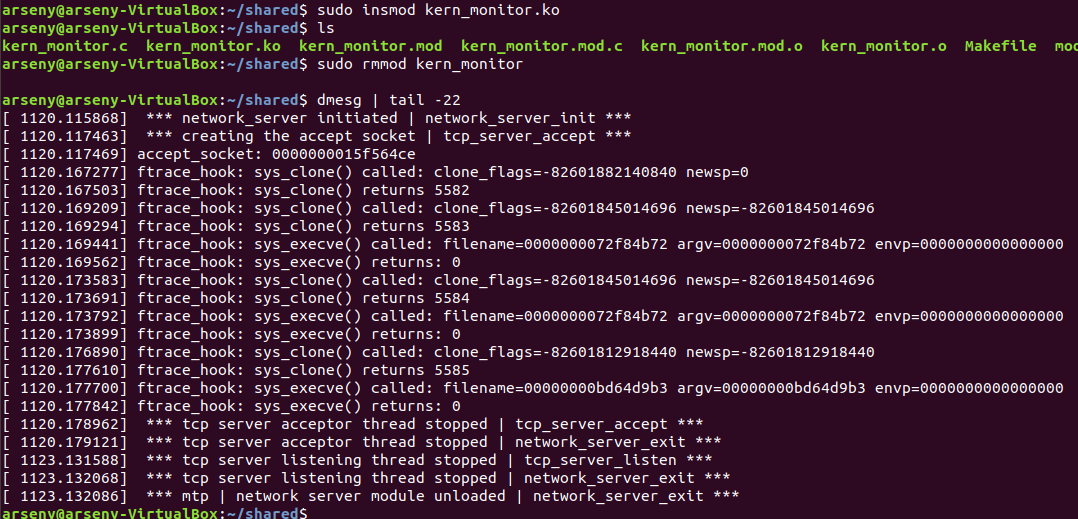
\includegraphics[width=1.0\textwidth]{img/res1}
	\caption{Результат работы модуля}
	\label{res1}
\end{figure}

\newpage
На рисунках \ref{res2} и \ref{res3} можно увидеть как клиент получает информацию о системных вызовах через сервер.

\begin{figure}[h!]
	\centering
	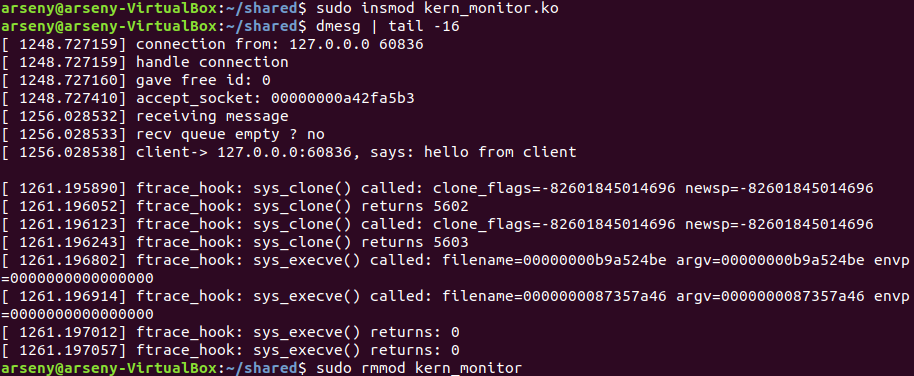
\includegraphics[width=1.0\textwidth]{img/res2}
	\caption{Взаимодействия между сервером модуля и клиентом}
	\label{res2}
\end{figure}

\begin{figure}[h!]
	\centering
	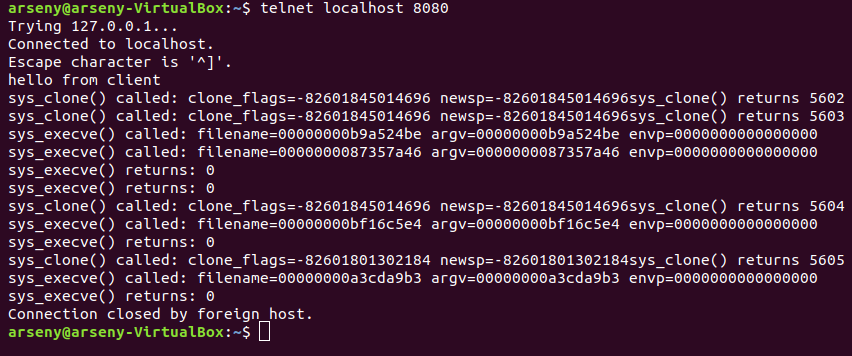
\includegraphics[width=1.0\textwidth]{img/res3}
	\caption{Взаимодействия между сервером модуля и клиентом}
	\label{res3}
\end{figure}

%\chapter{Заключение}
%\label{cha:research}
%\section{Время дизеринга раличных алгоритмов}

%В данном разделе проводятся вычислительные эксперименты.

%%% Local Variables:
%%% mode: latex
%%% TeX-master: "rpz"
%%% End:
